\documentclass[a4paper]{article}

\usepackage{a4wide}
\usepackage{amssymb}
\usepackage{hyperref}
\usepackage{subcaption}
\usepackage[numbers]{natbib}

\usepackage{tikz}
\tikzset{>=latex}

\newcommand{\vertex}[4][1.0]{
    \coordinate (#2) at (#3,#4);
    \filldraw (#2) circle (#1*0.05);
}
\newcommand\rectangle[4]{
    \draw (#1,#2) rectangle (#3,#4);
    \draw[dashed,gray] (#1,#2) -- (#3,#4);
    \draw[dashed,gray] (#1,#4) -- (#3,#2);
}

\title{Implementing Planar L-Drawings of Bimodal Triangulated Graphs}
\date{\today}

\begin{document}

\maketitle

\begin{abstract}
    In their 2020 paper, \citet{ldrawing} present a linear-time algorithm
    for constructing planar L-drawings of bimodal graphs.
    We implement and evaluate their algorithm.
    To this end, we also implement an algorithm for drawing rectangular duals
    \cite{dual} and for sampling plane triangulations \cite{sampling}.
    Our implementation realizes the theoretical linear running times.
    Furthermore, we develop an easy-to-implement algorithm that decomposes a
    graph into its 4-connected components.
    Finally, we point out flaws in the papers on planar L-drawings and
    rectangular duals.
\end{abstract}

\section{Introduction}
L-drawings for directed graphs were first introduced by \citet{ogldrawing} for
their increased readability of vertices with high degree.
In an L-drawing, vertices are drawn on distinct $x$- and $y$- coordinates, and a
directed edge from vertex $v$ to vertex $w$ is drawn as a 1-bend polyline
consisting of a vertical segment incident to $v$ and a horizontal segment
incident to $w$.
An example of an L-drawing can be seen in Figure \ref{fig:ldrawing:planar}.
\citet{npcomplete} focused on upward-planar L-drawings and gave a linear-time
algorithm for finding such a drawing if the embedding is fixed and admits an
upward-planar L-drawing.
\citet{ldrawing} finally showed that every bimodal graph without 2-cycles admits
a planar L-drawing, however not always an upward-planar one.
Their approach is based on rectangular duals.
An example of a rectangular dual can be seen in Figure
\ref{fig:ldrawing:rectdual}.
They leave it as an open problem whether all bimodal graphs \textit{with}
2-cycles admit a planar L-drawing.

\begin{figure}[ht]
    \center
    \begin{subfigure}{0.32\textwidth}
        \center
        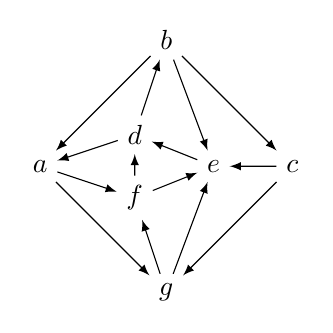
\begin{tikzpicture}[scale=0.8]
            \draw[draw=none,use as bounding box] (-0.2,-0.2) rectangle (4.2,4.2);
            \node (a) at (0,2){$a$};
            \node (b) at (2,4){$b$};
            \node (c) at (4,2){$c$};
            \node (d) at (1.5,2.5){$d$};
            \node (e) at (2.75,2){$e$};
            \node (f) at (1.5,1.5){$f$};
            \node (g) at (2,0){$g$};
            \draw[->] (a) -- (f);
            \draw[->] (a) -- (g);
            \draw[->] (b) -- (a);
            \draw[->] (b) -- (c);
            \draw[->] (b) -- (e);
            \draw[->] (c) -- (e);
            \draw[->] (c) -- (g);
            \draw[->] (d) -- (a);
            \draw[->] (d) -- (b);
            \draw[->] (e) -- (d);
            \draw[->] (f) -- (d);
            \draw[->] (f) -- (e);
            \draw[->] (g) -- (e);
            \draw[->] (g) -- (f);
        \end{tikzpicture}
        \caption{Straight-line}
    \end{subfigure}
    \hfill
    \begin{subfigure}{0.32\textwidth}
        \center
        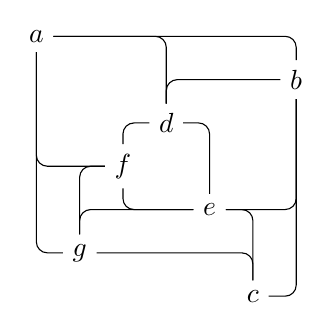
\begin{tikzpicture}[scale=0.55]
            \draw[draw=none,use as bounding box] (-0.2,-0.2) rectangle (6.2,6.2);
            \node (a) at (0,6){$a$};
            \node (b) at (6,5){$b$};
            \node (c) at (5,0){$c$};
            \node (d) at (3,4){$d$};
            \node (e) at (4,2){$e$};
            \node (f) at (2,3){$f$};
            \node (g) at (1,1){$g$};
            \draw[rounded corners] (a) |- (f);
            \draw[rounded corners] (a) |- (g);
            \draw[rounded corners] (b) |- (a);
            \draw[rounded corners] (b) |- (c);
            \draw[rounded corners] (b) |- (e);
            \draw[rounded corners] (c) |- (e);
            \draw[rounded corners] (c) |- (g);
            \draw[rounded corners] (d) |- (a);
            \draw[rounded corners] (d) |- (b);
            \draw[rounded corners] (e) |- (d);
            \draw[rounded corners] (f) |- (d);
            \draw[rounded corners] (f) |- (e);
            \draw[rounded corners] (g) |- (e);
            \draw[rounded corners] (g) |- (f);
        \end{tikzpicture}
        \caption{Planar L-drawing}
        \label{fig:ldrawing:planar}
    \end{subfigure}
    \hfill
    \begin{subfigure}{0.32\textwidth}
        \center
        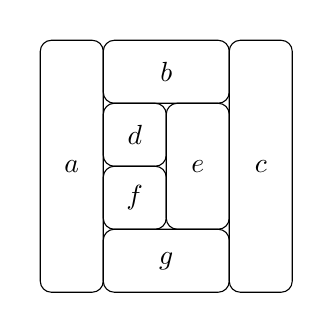
\begin{tikzpicture}[scale=0.8]
            \draw[draw=none,use as bounding box] (-0.2,-0.2) rectangle (4.2,4.2);
            \draw[rounded corners] (0,0) rectangle node{$a$} (1,4);
            \draw[rounded corners] (1,3) rectangle node{$b$} (3,4);
            \draw[rounded corners] (3,0) rectangle node{$c$} (4,4);
            \draw[rounded corners] (1,2) rectangle node{$d$} (2,3);
            \draw[rounded corners] (2,1) rectangle node{$e$} (3,3);
            \draw[rounded corners] (1,1) rectangle node{$f$} (2,2);
            \draw[rounded corners] (1,0) rectangle node{$g$} (3,1);
        \end{tikzpicture}
        \caption{Rectangular dual}
        \label{fig:ldrawing:rectdual}
    \end{subfigure}
    \caption{Various drawings of a graph}
    \label{fig:ldrawing}
\end{figure}

In this report, we implement the algorithm for planar L-drawings of bimodal
graphs, as well as the algorithms it uses as subroutines, and evaluate it on
sampled \cite{sampling} input graphs.
The algorithm for planar L-drawings involves decomposing a graph into
its 4-connected components.
To this end we describe an algorithm, which is comparably easy to implement and
yields the desired output directly.
Our method follows a similar approach as the left-right planarity test, as
described by \citet{lrpt}.

The remainder of this work is organized as follows:
Section \ref{sec:prelim} lays out all necessary definitions.
The algorithms used are described in Section \ref{sec:algo}.
We describe the experimental setup in Section \ref{sec:setup} and give the
experimental results in Section \ref{sec:results}.
In Section \ref{sec:other}, we correct some minor faults we found in the used
algorithms.
We conclude with open problems in Section \ref{sec:end}.

\section{Preliminaries}\label{sec:prelim}
\subsection{Graphs}
An \emph{undirected graph} $G = (V,E)$ consists of a \emph{vertex} set $V$ and
a set of \emph{undirected edges} $E \subseteq \{\{v,w\} \mid v,w \in V, v \not=
w\}$.
A \emph{directed graph} $G = (V,E)$ consists of a \emph{vertex} set $V$ and a
set of \emph{directed edges} $E \subseteq \{(v,w) \mid v,w \in V, v \not= w\}$.
We leave out \emph{directed} and \emph{undirected} whenever it is clear from
context.
Given an edge $e = (v,w)$, we say
$v$ and $w$ are the end points of $e$,
$v$ is the \emph{tail} of $e$,
$w$ is the \emph{head} of $e$.
$e$ is an \emph{outgoing} edge of $v$,
$e$ is an \emph{incoming} edge of $w$.
$v$ and $w$ are \emph{neighbors} or \emph{adjacent}.
An edge is \emph{incident} to its endpoints,
and its endpoints are \emph{incident} to the edge.
The degree $deg(v)$ of a vertex $v$ is the number of edges incident to $v$.

\subsection{Connectivity}
A \emph{directed $(v_0,v_l)$-path} of length $l$ in a directed graph $G$ is a
sequence $\langle v_0,e_1,v_1,e_2,\dots,e_l,v_l \rangle$ of vertices $v_i$ and
edges $e_i$, such that $e_i = (v_{i-1},v_i)$ for $i \in \{1,\dots,l\}$.
An \emph{undirected $(v_0,v_l)$-path} of length $l$ in a directed graph $G$ is
a sequence $\langle v_0,e_1,v_1,e_2,\dots,e_l,v_l \rangle$ of vertices $v_i$ and
edges $e_i$, such that $e_i = (v_{i-1},v_i)$ or $e_i = (v_i,v_{i-1})$ for $i \in
\{1,\dots,l\}$.
A directed (resp. undirected) $(v_0,v_0)$-path of length $l$ is called a
directed (resp. undirected) \emph{$l$-cycle}.
We identify a path with the sequence of its vertices or edges.
$G$ is \emph{connected} if for each pair of vertices $v,w \in V$ there is an
undirected $(v,w)$-path in $G$.
$G \setminus S$ is the graph $G$ with all vertices from $S$ along with their
incident edges removed.
$G$ is \emph{$k$-connected} if there is no set $S \subseteq V$ of $k-1$ vertices
such that $G \setminus S$ is disconnected.
If there is such a set $S$, it is called a separating \emph{$(k-1)$-tuple}.
A separating 3-tuple is also referred to as \emph{separating triple} or, if
there are edges between its members, \emph{separating triangle}.
A \emph{tree} is a connected undirected graph that contains no cycle.
In a tree vertices of degree 1 are called \emph{leaves}.

\subsection{Planarity}
A \emph{drawing} of $G$ is a mapping of the vertices and edges of $G$ into the
Euclidean plane; often vertices are drawn as points and edges as lines.
We identify vertices and edges with their drawings.
If the cyclic order of edges around each vertex is given, we call it an
\emph{embedding} of $G$.
A drawing (with points and lines) is \emph{planar} if edges only intersect in
common end points.
An embedding of $G$ is \emph{planar} if there is a planar drawing of $G$
respecting that embedding.
A graph is \emph{planar} if it has a planar embedding.
A planar drawing divides the plane into regions; these regions are called
\emph{faces} of the corresponding plane graph.
The unbounded face is called the \emph{outer face}.
All other faces are called \emph{inner faces}.
A graph together with a planar embedding and a fixed outer face is called a
\emph{plane} graph.
The \emph{degree} of a face is the number of half-edges that form its boundary.
In 2-connected graphs this is equal to the number of vertices that lie on its
boundary.
A graph is \emph{triangulated} if every face has degree $3$.
A graph is \emph{internally triangulated} if every inner face has degree
$3$.
A vertex $v$ in a plane directed graph is \emph{$k$-modal} ($mod(v) = k$) if in
the embedding around $v$ there are exactly $k$ pairs of consecutive edges that
are neither both incoming nor both outgoing.
A plane directed graph is \emph{$k$-modal} if $mod(v) \leq k$ for each of its
vertices $v$.
A $2$-modal graph is also referred to as \emph{bimodal}.

\subsection{L-Drawings}
An \emph{L-drawing} of a directed graph $G = (V,E)$ is a mapping of the vertices
of $G$ to points into the plane such that no two vertices are assigned the same
$x$- or $y$-coordinates.
In other words an L-drawing is a pair of injective functions $x,y : V \to
\mathbb N$.
A directed edge $(v,w)$ is then drawn as the polyline $(x(v),y(v)) - (x(v),y(w))
- (x(w),y(w))$, that is a vertical segment incident to $v$, followed by a
horizontal segment incident to $w$.
For each vertex, we consider four \emph{ports}, North, East, South, and West.
In an L-drawing, an edge is assigned to the North (resp. South) port of its tail
if it leaves it to the top (resp. bottom), and to the East (resp. West) port of
its head if it enters it from the right (resp. left).
An L-drawing is \emph{planar} if no two edges cross, however they may share a
subsegment at a common endpoint.

\subsection{Rectangular Duals}
An \emph{irreducible trianglulation} is a 4-connected internally triangulated
plane graph with an outer face of degree $4$.
A \emph{rectangular tiling} is a partition of a rectangle into smaller
rectangles such that no four rectangles touch in the same point.
A rectangular tiling $T$ is called a \emph{rectangular dual} of a graph $G$ if
there is a one-to-one correspondence between the rectangles in $T$ and vertices
of $G$ such that there exists an edge between two vertices iff the corresponding
rectangles touch.

\section{Algorithms}\label{sec:algo}
\subsection{4-Connected Components}\label{sec:algo:decompose}
The first task is to find the 4-connected components of the triangulated input
graph.
To this end, \citet{ldrawing} cite \citet{kant}, who described a method for this
problem.
The main idea there is to list all triangles, as described by
\citet{triangles}, select the separating ones among them,
and then to order them, either from the inside out or from
the outside in, such that one can split the graph along each separating triangle
in constant time while keeping track of which edge is incident to which copy of
the original vertex.
This splitting step is not well documented and rather involved; therefore we
will propose a different method of ordering the separating triangles, namely
only from the inside out.
This way the splitting need only be done in linear time to accomplish the
decomposing in linear time.
The input graph is considered to be undirected for this step, and any direction
defined on the edges is defined during a traversal of the graph.
For examples see Figure \ref{fig:lowpoint}.

\begin{figure}[hp]
    \center
    \begin{subfigure}{0.37\textwidth}
        \center
        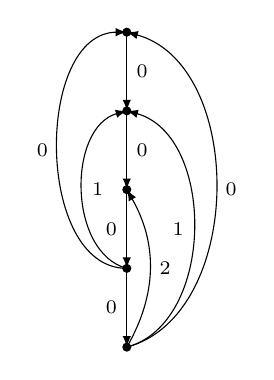
\begin{tikzpicture}
            \vertex 0 0 4
            \vertex 1 0 3
            \vertex 2 0 2
            \vertex 3 0 1
            \vertex 4 0 0
            \draw[->] (0) -- (1) node[midway,right,font=\scriptsize] {0};
            \draw[->] (1) -- (2) node[midway,right,font=\scriptsize] {0};
            \draw[->] (2) -- (3) node[midway,left,font=\scriptsize] {0};
            \draw[->] (3) -- (4) node[midway,left,font=\scriptsize] {0};
            \draw[->] (3) to[out=165,in=195] node[midway,right,font=\scriptsize] {1} (1);
            \draw[->] (3) to[out=180,in=180] node[midway,left,font=\scriptsize] {0} (0);
            \draw[->] (4) to[out=60,in=300] node[midway,right,font=\scriptsize] {2} (2);
            \draw[->] (4) to[out=15,in=345] node[midway,left,font=\scriptsize] {1} (1);
            \draw[->] (4) to[out=15,in=345] node[midway,right,font=\scriptsize] {0} (0);
        \end{tikzpicture}
        \caption{Edges with their \textsc{lowpoint}s}
        \label{fig:lowpoint:lowpoint}
    \end{subfigure}
    \hfill
    \begin{subfigure}{0.5\textwidth}
        \center
        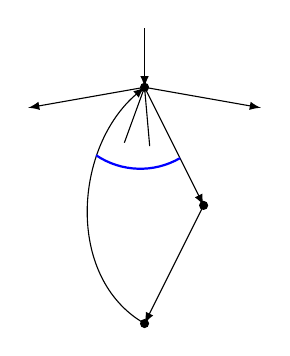
\begin{tikzpicture}[scale=1.5]
            \vertex[0.67] p 0 2
            \vertex[0.67] v {0.5} 1
            \vertex[0.67] w 0 0
            \draw[<-] (p) -- +(0,0.5);
            \draw[->] (p) -- +(-10:1);
            \draw[->] (p) -- +(180+10:1);
            \draw[->] (p) -- (v);
            \draw[->] (v) -- (w);
            \draw[->] (w) to[out=150,in=220] (p);
            \draw[blue,thick] (p) +(0.3,-0.6) arc (300:236:0.671);
            \draw (p) -- +(250:0.5);
            \draw (p) -- +(275:0.5);
        \end{tikzpicture}
        \caption{A back edge with $\textsc{returnSide} = \mathrm{Left}$ and
        $\textsc{angularDistance} = 2$}
        \label{fig:lowpoint:angularDistance}
    \end{subfigure}

    \vspace{1cm}
    \begin{subfigure}{0.5\textwidth}
        \center
        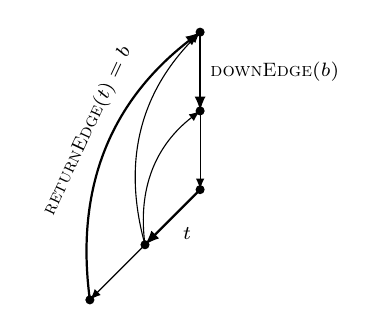
\begin{tikzpicture}
            \vertex 0 2 4
            \vertex 1 2 3
            \vertex 2 2 2
            \vertex 3 {1.3} {1.3}
            \vertex 4 {0.6} {0.6}
            \draw[->,thick] (0) -- node[font=\scriptsize,right]
            {$\textsc{downEdge}(b)$} (1);
            \draw[->] (1) -- (2);
            \draw[->,thick] (2) -- node[font=\scriptsize,below right] {$t$} (3);
            \draw[->] (3) -- (4);
            \draw[->] (3) to[bend left] (1);
            \draw[->] (3) to[bend left] (0);
            \draw[->,thick] (4) to[bend left]
            node[label={[font=\scriptsize,rotate=65]$\textsc{returnEdge}(t)=b$}]
            {} (0);
        \end{tikzpicture}
        \caption{A tree edge, its \textsc{returnEdge} and a \textsc{downEdge}}
        \label{fig:lowpoint:returnEdge}
    \end{subfigure}
    \hfill
    \begin{subfigure}{0.45\textwidth}
        \center
        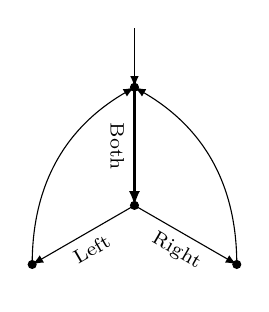
\begin{tikzpicture}[scale=1.5]
            \vertex[0.67] p 1 2
            \vertex[0.67] c 1 1
            \vertex[0.67] l {0.134} {0.5}
            \vertex[0.67] r {1.866} {0.5}
            \draw[<-] (p) -- +(0,0.5);
            \draw[->,thick] (p) -- node[font=\scriptsize,rotate=-90,below] {Both} (c);
            \draw[->] (c) -- node[font=\scriptsize,below,rotate=30] {Left} (l);
            \draw[->] (c) -- node[font=\scriptsize,below,rotate=-30] {Right} (r);
            \draw[->] (l) to[bend left] (p);
            \draw[->] (r) to[bend right] (p);
        \end{tikzpicture}
        \caption{A tree edge with $\textsc{returnSide} = \mathrm{Both}$}
        \label{fig:lowpoint:both}
    \end{subfigure}

    \vspace{1cm}
    \begin{subfigure}{\textwidth}
        \center
        \begin{tabular}{c|cc}
            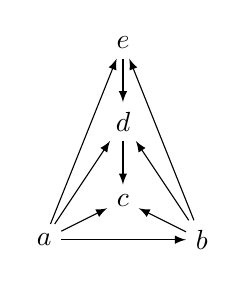
\begin{tikzpicture}
                \node (a) at (0,0.5) {$a$};
                \node (b) at (2,0.5) {$b$};
                \node (c) at (1,1) {$c$};
                \node (d) at (1,2) {$d$};
                \node (e) at (1,3) {$e$};
                \draw[->] (a) -- (b);
                \draw[->] (a) -- (c);
                \draw[->] (a) -- (d);
                \draw[->] (a) -- (e);
                \draw[->] (b) -- (c);
                \draw[->] (b) -- (d);
                \draw[->] (b) -- (e);
                \draw[->] (d) -- (c);
                \draw[->] (e) -- (d);
            \end{tikzpicture}
            &
            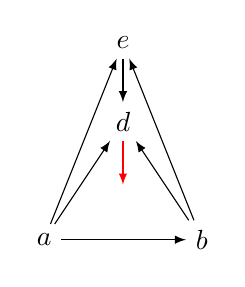
\begin{tikzpicture}
                \node (a) at (0,0.5) {$a$};
                \node (b) at (2,0.5) {$b$};
                \node (c) at (1,1) {\phantom{$c$}};
                \node (d) at (1,2) {$d$};
                \node (e) at (1,3) {$e$};
                \draw[->] (a) -- (b);
                \draw[->] (a) -- (d);
                \draw[->] (a) -- (e);
                \draw[->] (b) -- (d);
                \draw[->] (b) -- (e);
                \draw[->,red] (d) -- (c);
                \draw[->] (e) -- (d);
            \end{tikzpicture}
            &
            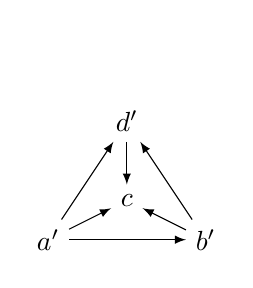
\begin{tikzpicture}
                \node (a) at (0,0.5) {$a'$};
                \node (b) at (2,0.5) {$b'$};
                \node (c) at (1,1) {$c$};
                \node (d) at (1,2) {$d'$};
                \node (e) at (1,3) {\phantom{$e$}};
                \draw[->] (a) -- (b);
                \draw[->] (a) -- (c);
                \draw[->] (a) -- (d);
                \draw[->] (b) -- (c);
                \draw[->] (b) -- (d);
                \draw[->] (d) -- (c);
            \end{tikzpicture}
        \end{tabular}
        \caption{Before and after splitting along the separating triangle with
        virtual edge}
        \label{fig:lowpoint:split}
    \end{subfigure}
    \caption{Examples illustrating the decomposition step}
    \label{fig:lowpoint}
\end{figure}

\medskip\noindent
\textbf{Listing separating triples.}
Here, we make use of the fact that in a plane triangulation all separating
triples are separating triangles.
Therefore, it suffices to list all triangles \cite{triangles} and then select
those triangles $u,v,w$ where $v$ and $w$ do not appear consecutively in the
adjacency list of $u$.

\medskip\noindent
\textbf{Ordering separating triangles.}
This step is heavily inspired by the left-right planarity test \cite{lrpt}.
First, we perform a depth-first search on the undirected input graph, starting
from one of the outer vertices $r$. During this process we take note of the
following:
\begin{itemize}
    \item
        the direction that each edge was traversed in
    \item
        for each edge $e$ whether it is a tree edge (its head was newly
        discovered when traversing $e$) or a back edge (its head had already
        been discovered)
    \item
        $\textsc{depth}(v)$ of each vertex $v$, the length of the $(r,v)$-path
        along tree edges
    \item
        $\textsc{parentEdge}(v)$ of each vertex $v$, the edge along which $v$
        was first discovered.
        For $r$, this is a virtual edge between the edges to its two neighbors
        on the outer face.
    \item for each back edge $e$:
        \begin{itemize}
            \item
                $\textsc{lowpoint}(e) = \textsc{depth}(e.head)$
            \item
                $\textsc{downEdge}(e) = (p,c)$
                if $p = e.head, t = e.tail$
                and $\langle p,c,\dots,t \rangle$ is the unique $(p,t)$-path along tree
                edges.
            \item
                $\textsc{returnSide}(e) \in \{\mathrm{Left}, \mathrm{Right}\}$
                is the side on
                which $e$ enters its head $p$: Left if the clockwise
                order of edges around $p$ is $\textsc{parentEdge}(p)$,
                $\textsc{downEdge}(e)$, $e$; Right if it is
                $\textsc{parentEdge}(p)$, $e$, $\textsc{downEdge}(e)$.
            \item
                $\textsc{angularDistance}(e)$ is the number of edges that appear in the
                adjacency list of $e.head$ in clockwise order\dots
                \begin{itemize}
                    \item
                        if $\textsc{returnSide}(e) = \mathrm{Left}$:
                        \dots{}between $\textsc{downEdge}(e)$ and
                        $e$.
                    \item
                        if $\textsc{returnSide}(e) = \mathrm{Right}$:
                        \dots{}between $e$ and
                        $\textsc{downEdge}(e)$.
                \end{itemize}
        \end{itemize}
    \item for each tree edge $e$:
        \begin{itemize}
            \item
                $\textsc{returnEdge}(e)$:
                Consider directed paths
                $\langle t_1,\dots,t_l,b \rangle$ where $t_i$
                are tree edges, $b$ is a back edge and $t_1 = e$.
                Select those with minimal $\textsc{lowpoint}(b)$ among them.
                Then select those with maximal $\textsc{angularDistance}(b)$ among them.
                Finally, select any path from these and let
                $\textsc{returnEdge}(e) = b$ of that path.
            \item
                $\textsc{lowpoint}(e) = \textsc{lowpoint}(\textsc{returnEdge}(e))$
            \item
                $\textsc{returnSide}(e)$:
                If, when finding $\textsc{returnEdge}(e)$, not all paths
                $\langle t_1, \dots, t_l, b \rangle$ with
                minimal $\textsc{lowpoint}(b)$ had the same
                $\textsc{returnSide}(b)$, then let $\textsc{returnSide}(e) =
                \mathrm{Both}$.
                Otherwise let $\textsc{returnSide}(e) =
                \textsc{returnSide}(\textsc{returnEdge}(e))$.
            \item
                $\textsc{angularDistance}(e) = \textsc{angularDistance}(\textsc{returnEdge}(e))$
        \end{itemize}
\end{itemize}
With this information, we define for each vertex $v$ a partial ordering $\prec$
of its outgoing edges:
\begin{itemize}
    \item $e_1 \prec e_2$ if $\textsc{lowpoint}(e_1) > \textsc{lowpoint}(e_2)$
    \item $e_1 \prec e_2$ if $\textsc{lowpoint}(e_1) = \textsc{lowpoint}(e_2)$,
        $\textsc{returnSide}(e_1) = \textsc{returnSide}(e_2)$ and
        $\textsc{angularDistance}(e_1) < \textsc{angularDistance}(e_2)$
    \item $e_1 \prec e_2$ if $\textsc{lowpoint}(e_1) = \textsc{lowpoint}(e_2)$,
        $\textsc{returnSide}(e_1) \not= \textsc{returnSide}(e_2)$,
        $e_1$ is a back edge and $e_2$ is a tree edge
    \item $e_1 \prec e_2$ if $\textsc{returnSide}(e_2) = \mathrm{Both}$.
        Note that there is at most one such edge $e_2$.
\end{itemize}
After sorting the outgoing edges of each vertex according to this ordering
$\prec$, we
perform a second depth-first search of the graph, following the order of edges.
During this second traversal of the graph, we take note of the order in which
the separating triangles are discovered.
For this purpose, we consider a separating triangle to be discovered once all
three of its edges have been traversed.

If several separating triangles $T_1, \dots, T_n$ are discovered at the same
time, they share an edge $\{v,w\}$ and have distinct third vertices $u_1, \dots,
u_n$.
For each triangle $T_i$ consider the vertex $x$ on it that has the lowest
\textsc{depth}; $\textsc{parentEdge}(x)$ is on the outside of $T_i$.
Now sort $T_1, \dots, T_n$ according to the number of neighbors $v$ (or $w$) has
on the inside of the respective triangle.
The triangle with the least neighbors of $v$ (or $w$) on its inside is the
innermost.
We consider $T_1, \dots, T_n$ to be discovered in this sorted order, from the
innermost to the outermost.

The order in which the separating triangles are discovered here is the order in
which they will be processed in the next step.

\medskip\noindent
\textbf{Splitting along separating triangles.}
For each separating triangle with vertices $u,v,w$, make copies $u',v',w'$ of
its three vertices and add the three edges $\{u',v'\}, \{v',w'\}, \{w',u'\}$.
Transfer to $u'$ the edges incident to $u$ on the inside of the triangle;
analogously for $v$ and $w$.

If the edges $\{u,v\}$ and $\{u,w\}$ are both incoming (resp. outgoing) in the
original graph and $u'$ has now an outgoing (resp. incoming) edge, add a virtual
outgoing (resp. incoming) edge to $u$ between $\{u,v\}$ and $\{u,w\}$;
analogously for $v$ and $w$.
This is done to preserve the bimodality of $u$ in the outer 4-connected
component for the port assignment.

\medskip\noindent
\textbf{Identifying 4-connected components.}
Finally, identify the connected components of the resulting graph, for example
using breadth-first search.
These are the 4-connected components of the original graph since the 4-connected
components have been turned into connected components during the splitting step.

If we take for each separating triangle $u,v,w$ the connected component with the
outer face $u',v',w'$ in the reverse splitting order, it holds that the
component containing $u,v,w$ will appear before the component with the outer
face $u',v',w'$.

\medskip\noindent
\textbf{Linear running time.}
During the first depth-first search, do not list the paths $\langle t_1, \dots,
t_l, b \rangle$ explicitly, but instead keep track of the back edge $b$ with
minimal \textsc{lowpoint} and maximal \textsc{angularDistance} in the subtree
that is currently being traversed.
When popping a tree edge $t$ from the depth-first search stack, we will have
$\textsc{returnEdge}(t) = b$.
To find $\textsc{returnSide}(t)$, take note if a back edge with
\textsc{lowpoint} and \textsc{angularDistance} equal to $b$ is found in the
subtree.

Do not find the path $\langle p, c, \dots, t \rangle$ explicitly after
traversing the subtree rooted at $c$, but instead
save the edge $(p,c)$ as $\textsc{activeChildEdge}(p)$ while the subtree rooted
at $c$ is being traversed.

Use bucket sort to sort the outgoing edges of
each vertex before the second depth-first traversal.

\subsection{Rectangular Duals}
The next task is to construct rectangular duals of the 4-connected components.
For this, we use the algorithm presented in \citet{dual}, which takes as input
an irreducible trianglulation.

\medskip\noindent
\textbf{Finding a $(3,1)$-ordering.}
The first step is to find an ordering of paths in the graph, such that each of
these paths has at least $3$ predecessors in the ordering (neighboring vertices
that appear before it) and at least one successor.
Each of these paths may take one of the two forms shown in Figure
\ref{fig:dual:ordering}.

\medskip\noindent
\textbf{Constructing the rectangular dual.}
Each of the paths is then placed to the right of its leftmost predecessor, to
the left of its rightmost predecessor and above all other predecessors, as can
be seen in Figure \ref{fig:dual:dual}.

\begin{figure}[ht]
    \center
    \begin{subfigure}{0.26\textwidth}
        \center
        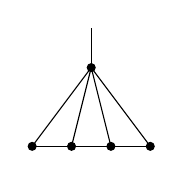
\begin{tikzpicture}
            \coordinate (v) at (1.25,1){};
            \coordinate (p1) at (0.5,0){};
            \coordinate (p2) at (1,0){};
            \coordinate (p3) at (1.5,0){};
            \coordinate (p4) at (2,0){};
            \foreach \v in {v,p1,p2,p3,p4}
                \filldraw (\v) circle (0.05);
            \draw (v) -- +(0,0.5);
            \draw (p1) -- (v);
            \draw (p2) -- (v);
            \draw (p3) -- (v);
            \draw (p4) -- (v);
            \draw (p1) -- (p2);
            \draw (p2) -- (p3);
            \draw (p3) -- (p4);
        \end{tikzpicture}
        \quad
        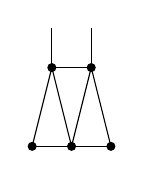
\begin{tikzpicture}
            \coordinate (v1) at (0.75,1){};
            \coordinate (v2) at (1.25,1){};
            \coordinate (p1) at (0.5,0){};
            \coordinate (p2) at (1,0){};
            \coordinate (p3) at (1.5,0){};
            \foreach \v in {v1,v2,p1,p2,p3}
                \filldraw (\v) circle (0.05);
            \draw (v1) -- +(0,0.5);
            \draw (v2) -- +(0,0.5);
            \draw (v1) -- (v2);
            \draw (p1) -- (v1);
            \draw (p2) -- (v1);
            \draw (p2) -- (v2);
            \draw (p3) -- (v2);
            \draw (p1) -- (p2);
            \draw (p2) -- (p3);
        \end{tikzpicture}
        \caption{Singleton and fan paths in the $(3,1)$-ordering}
        \label{fig:dual:ordering}
    \end{subfigure}
    \qquad
    \begin{subfigure}{0.59\textwidth}
        \center
        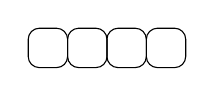
\begin{tikzpicture}[scale=0.5]
            \draw[rounded corners] (0,0) rectangle (1,1);
            \draw[rounded corners] (1,0) rectangle (2,1);
            \draw[rounded corners] (2,0) rectangle (3,1);
            \draw[rounded corners] (3,0) rectangle (4,1);
        \end{tikzpicture}
        \quad
        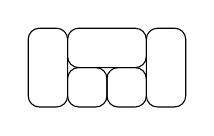
\begin{tikzpicture}[scale=0.5]
            \draw[rounded corners] (0,0) rectangle (1,2);
            \draw[rounded corners] (1,0) rectangle (2,1);
            \draw[rounded corners] (2,0) rectangle (3,1);
            \draw[rounded corners] (3,0) rectangle (4,2);
            \draw[rounded corners] (1,1) rectangle (3,2);
        \end{tikzpicture}
        \quad
        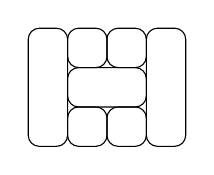
\begin{tikzpicture}[scale=0.5]
            \draw[rounded corners] (0,0) rectangle (1,3);
            \draw[rounded corners] (1,0) rectangle (2,1);
            \draw[rounded corners] (2,0) rectangle (3,1);
            \draw[rounded corners] (3,0) rectangle (4,3);
            \draw[rounded corners] (1,1) rectangle (3,2);
            \draw[rounded corners] (1,2) rectangle (2,3);
            \draw[rounded corners] (2,2) rectangle (3,3);
        \end{tikzpicture}
        \caption{Incremental drawing of the dual}
        \label{fig:dual:dual}
    \end{subfigure}
    \caption{The algorithm for drawing rectangular duals}
    \label{fig:dual}
\end{figure}

\subsection{Port Assignment}
The port assignment algorithm \cite{ldrawing} takes as input a 4-connected
bimodal triangulation and an L-drawing of its outer face.
First, split one of the edges on the outer face by inserting a dummy vertex into
it.
Now the outer face has degree 4; therefore the graph is now an irreducible
triangulation, for which a rectangular dual can be constructed.

After drawing the rectangular dual, we place each vertex in the center of its
rectangle (Figure \ref{fig:pa:dual}).
The North port of a vertex is then to its top left, the East port to its top
right, the South port to its bottom right, and the West port to its bottom left.
The edges are routed parallel to the diagonals of the rectangles (Figure
\ref{fig:pa:pa}).
An outgoing edge that leaves the rectangle of a vertex to the top will be
assigned to its North port if possible, because that port points to the top
(left), unlike the South port, which points to the bottom (right).
Recall that outgoing edges may only be assigned to the North or South port.
We handle incoming edges and edges on other sides of the rectangle
analogously.

\begin{figure}[ht]
    \center
    \begin{subfigure}{0.32\textwidth}
        \center
        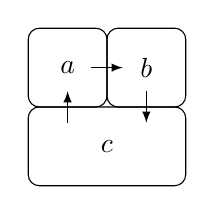
\begin{tikzpicture}
            \draw[rounded corners] (1,1) rectangle node {$c$} (3,2);
            \draw[rounded corners] (1,2) rectangle node {$a$} (2,3);
            \draw[rounded corners] (2,2) rectangle node {$b$} (3,3);
            \draw[->] (1.5,1.8) -- (1.5,2.2);
            \draw[<-] (2.5,1.8) -- (2.5,2.2);
            \draw[->] (1.8,2.5) -- (2.2,2.5);
        \end{tikzpicture}
        \caption{Rectangular dual}
        \label{fig:pa:dual}
    \end{subfigure}
    \hfill
    \begin{subfigure}{0.32\textwidth}
        \center
        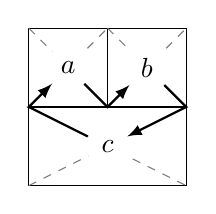
\begin{tikzpicture}
            \rectangle 1 1 3 2
            \rectangle 1 2 2 3
            \rectangle 2 2 3 3
            \node[circle,fill=white] (v) at (2,1.5)  {$c$};
            \node[circle,fill=white] (a) at (1.5,2.5){$a$};
            \node[circle,fill=white] (b) at (2.5,2.5){$b$};
            \draw[->,thick] (v) -- (1,2) -- (a);
            \draw[->,thick] (a) -- (2,2) -- (b);
            \draw[->,thick] (b) -- (3,2) -- (v);
        \end{tikzpicture}
        \caption{Port assignment}
        \label{fig:pa:pa}
    \end{subfigure}
    \hfill
    \begin{subfigure}{0.32\textwidth}
        \center
        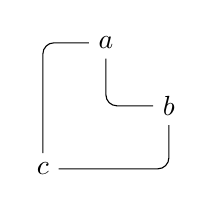
\begin{tikzpicture}[scale=0.8]
            \tikzset{>=latex}
            \node (v) at (2,2){$c$};
            \node (a) at (3,4){$a$};
            \node (b) at (4,3){$b$};
            \draw[rounded corners] (v) |- (a);
            \draw[rounded corners] (b) |- (v);
            \draw[rounded corners] (a) |- (b);
        \end{tikzpicture}
        \caption{L-drawing}
        \label{fig:pa:ldrawing}
    \end{subfigure}
    \caption{From rectangular dual to L-drawing}
    \label{fig:pa}
\end{figure}

After the port assignment in one 4-connected component $C$ is complete, the same
can be done for all other 4-connected components whose outer face is an inner
face of $C$.
This way, we execute a preorder traversal of the tree of 4-connected components.
Note that in our implementation this tree is not built explicitly, but instead
its nodes are given in preorder in the order of separating triangles
(Section \ref{sec:algo:decompose}).

When all ports in the graph have been assigned, the edges imply an order of the
vertices in $x$- and $y$- direction.
For example, if an edge $(v,w)$ has been assigned to the North port of $v$ and
to the West port of $w$, $v$ must be drawn below and to the left of $w$.
This order can be found through topological ordering.

\subsection{Sampling Triangulations}\label{sec:algo:sampling}
To test the above algorithms, we used a sampling algorithm that was developed by
\citet{sampling}.
It takes as input an integer $n$ and outputs a plane triangulation with $n+2$
vertices and $3n$ edges.
It randomly generates a bitstring of length $4n-2$ with $3n-1$ zeros and $n-1$
ones.
Using the cycle lemma \cite{cyclelemma}, it finds one of its cyclic shifts $s$
that has the property that each prefix $u$ of $s$ satisfies $3|u|_{\tt 1} -
|u|_{\tt 0} \geq -2$.

From this bitstring $s$ a tree is then constructed.
All inner (non-leaf) vertices in this tree are adjacent to exactly two leaves.
The construction works as follows:
The bitstring encodes a walk around the tree in counter-clockwise direction; a
{\tt 1} stands for a downwards edge connecting to inner vertices; a {\tt 0}
stands for a leaf if the current inner vertices does not have to adjacent leaves
yet, otherwise it stands for an upwards edge.
This way each inner edge appears twice in the encoding, each leaf edge only
once.
Such a tree constructed from a bitstring can be seen in Figure
\ref{fig:sample:tree}.

Next, walk around the graph, searching for two consecutive inner edges
followed by a leaf edge.
Whenever this configuration is encountered, attach the leaf edge to the first of
the three inner vertices that are incident to the three edges.
The result of this operation is shown in Figure \ref{fig:sample:closure}.

When such a configuration cannot be found anymore, each vertex on the outer face
will have exactly one incident leaf edge with the exception of two vertices
$a,b$ that still have two incident leaf edges.
Now add two more vertices $x,y$ in the outer face and connect all leaf edges
between $a$ and $b$ to $x$ and all leaf edges between $b$ and $a$ to $y$.
Finally, triangulate the outer face by adding the edge $\{x,y\}$ in the outer
face.
Figure \ref{fig:sample:done} shows the complete constructed graph.

\begin{figure}[ht]
    \center
    \begin{subfigure}{0.4\textwidth}
        \center
        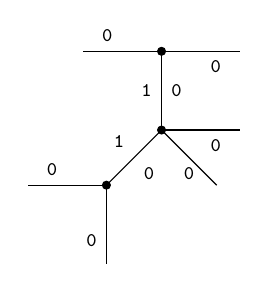
\begin{tikzpicture}
            \draw[draw=none,use as bounding box] (1.3,-0.7) rectangle (4,2.3);
            \coordinate (1) at (3,2){};
            \draw (1) -- node[above left,font=\scriptsize]{\tt 0} +(-1,0);
            \coordinate (2) at (3,1){};
            \draw (1) -- node[left,font=\scriptsize]{\tt 1} node[right,font=\scriptsize]{\tt 0} (2);
            \coordinate (3) at (2.3,0.3){};
            \draw (2) -- node[above left,font=\scriptsize]{\tt 1} node[below right,font=\scriptsize]{\tt 0} (3);
            \draw (3) -- node[above left,font=\scriptsize]{\tt 0} +(-1,0);
            \draw (3) -- node[below left,font=\scriptsize]{\tt 0} +(0,-1);
            \draw (2) -- node[below,font=\scriptsize]{\tt 0} +(0.7,-0.7);
            \draw (2) -- node[below right,font=\scriptsize]{\tt 0} +(1,0);
            \draw (1) -- node[below right,font=\scriptsize]{\tt 0} +(1,0);
            \foreach \v in {1,...,3}
                \filldraw (\v) circle (0.05);
        \end{tikzpicture}
        \caption{Tree with two leaves per inner vertex}
        \label{fig:sample:tree}
    \end{subfigure}
    \hfill
    \begin{subfigure}{0.35\textwidth}
        \center
        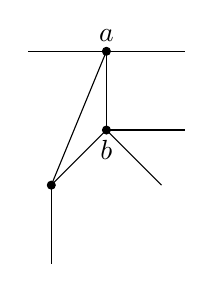
\begin{tikzpicture}
            \draw[draw=none,use as bounding box] (2,-0.7) rectangle (4,2.3);
            \coordinate (1) at (3,2){};
            \draw (1) -- +(-1,0);
            \coordinate (2) at (3,1){};
            \draw (1) -- (2);
            \coordinate (3) at (2.3,0.3){};
            \draw (2) -- (3);
            \draw (3) -- (1);
            \draw (3) -- +(0,-1);
            \draw (2) -- +(0.7,-0.7);
            \draw (2) -- +(1,0);
            \draw (1) -- +(1,0);
            \foreach \v in {1,...,3}
                \filldraw (\v) circle (0.05);
            \node[above] at (1) {$a$};
            \node[below] at (2) {$b$};
        \end{tikzpicture}
        \caption{After closing all triangles}
        \label{fig:sample:closure}
    \end{subfigure}
    \hfill
    \begin{subfigure}{0.23\textwidth}
        \center
        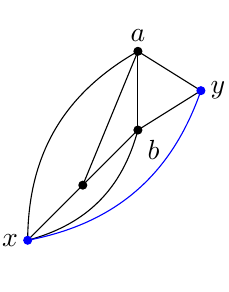
\begin{tikzpicture}
            \draw[draw=none,use as bounding box] (1.6,-0.7) rectangle (3.8,2.3);
            \coordinate (4) at (3.8,1.5){};
            \coordinate (5) at (1.6,-0.4){};
            \coordinate (1) at (3,2){};
            \draw (1) to[bend right] (5);
            \coordinate (2) at (3,1){};
            \draw (1) -- (2);
            \coordinate (3) at (2.3,0.3){};
            \draw (2) -- (3);
            \draw (3) -- (1);
            \draw (3) -- (5);
            \draw (2) to[bend left] (5);
            \draw (2) -- (4);
            \draw (1) -- (4);
            \draw[blue] (5) to[bend right] (4);
            \foreach \v in {1,...,3}
                \filldraw (\v) circle (0.05);
            \foreach \v in {4,5}
                \filldraw[blue] (\v) circle (0.05);
            \node[above] at (1) {$a$};
            \node[below right] at (2) {$b$};
            \node[right] at (4) {$y$};
            \node[left]  at (5) {$x$};
        \end{tikzpicture}
        \caption{Complete graph}
        \label{fig:sample:done}
    \end{subfigure}
    \caption{Example of the sampling algorithm for $n = 3, s = \tt0110000000$}
    \label{fig:sample}
\end{figure}

\section{Experimental Setup}\label{sec:setup}
We used the algorithm described in Section \ref{sec:algo:sampling} to sample
plane undirected triangulations for different values of $n$.
The edges of these graphs were then directed through an open ear
decomposition \cite{openear}.
This implies a bimodal embedding (upward-planar, even).
The resulting directed graph was drawn by the algorithm of \citet{ldrawing}.

To show the correctness of our implementation, we sampled 1000 graphs with
$n=1000$ and naively tested whether there are any crossings in the L-drawing
computed by our implementation.

To test the running time, we timed our program for sampled input graphs with
$n \in \{10^6, 2 \cdot 10^6, \dots, 10^7\}$.
All tests were executed on a 64-bit computer with 24 GB of DDR4-2133 RAM running
Ubuntu 20.04.2 LTS, in a single thread on a single core of an Intel i7-7700K CPU
@ 4.20 GHz.
The implementation was written in C++17 using the Standard Template Library and
compiled with g++ 9.3.0 set to the highest optimization level.
The running time of the sampling algorithm was measured using the {\tt time}
builtin of zsh 5.8.
The running times of the individual subroutines of the L-drawing algorithm were
measured using {\tt std::chrono::steady\_clock}.

\section{Test Results}\label{sec:results}
No intersections were found in the correctness test.

The running times of the sampling algorithm, including the open ear
decomposition can be seen in Figure \ref{fig:sampling}.
It is clear that the running time of our implementation is linear in $n$.

\begin{figure}[ht]
    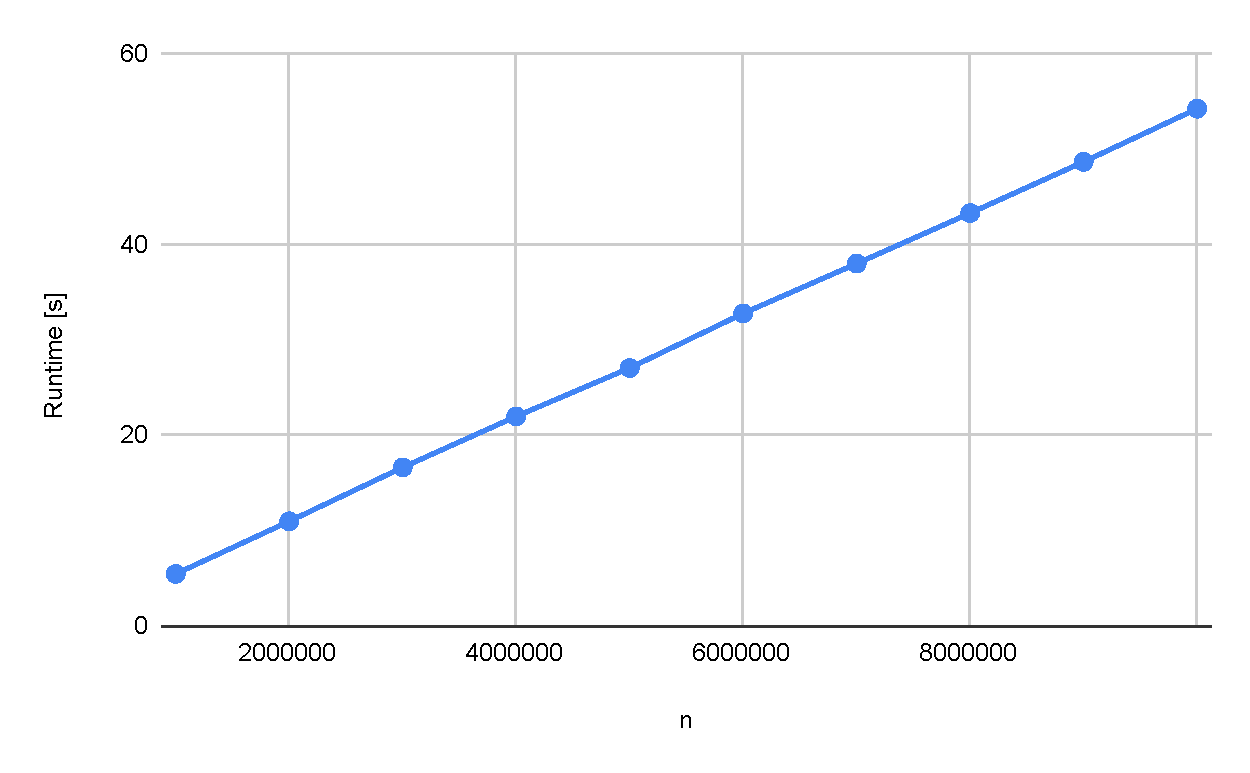
\includegraphics[width=\textwidth]{sampling.pdf}
    \caption{Running times for the sampling algorithm}
    \label{fig:sampling}
\end{figure}

Figure \ref{fig:results} shows the running times of our implementation of the
algorithm of \citet{ldrawing}.
The times for reading the input graph and writing the output drawing, for
decomposing the graph into its 4-connected components, for drawing the
rectangular dual of each 4-connected component, and for assigning each edge to
the ports of its endpoints are given separately.
The times are linear in $n$ as well.

\begin{figure}[ht]
    \center
    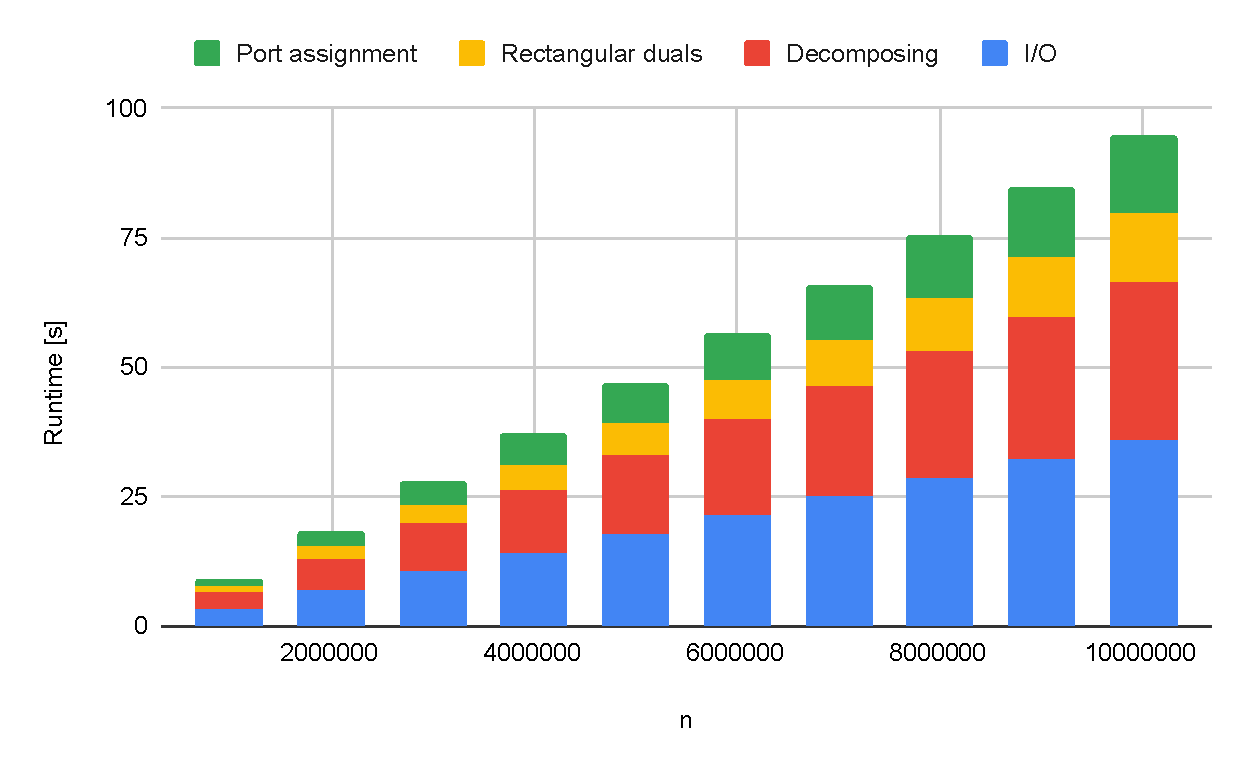
\includegraphics[width=\textwidth]{results.pdf}
    \caption{Running times for the L-drawing algorithm}
    \label{fig:results}
\end{figure}

\section{Other Results}\label{sec:other}
\subsection{Identifying Basic 2-Leg Centers for the (3,1)-ordering}
The configuration on the right of Figure \ref{fig:dual:ordering} is called a
\emph{fan}.
A fan is a simple path of vertices $c_1, \dots, c_k$ that are all adjacent to one
common predecessor $y$, which is called \emph{minimal 2-leg center}.
Additionally, the leftmost vertex $c_1$ of the path is adjacent to a predecessor
$l$ one to the left from the minimal 2-leg center, and the rightmost vertex
$c_k$ is adjacent to a predecessor $r$ one to the right from $y$.
A fan is picked whenever there is no singleton that can be picked.
\citet{dual} define a \emph{2-leg center} as an inner vertex that is adjacent to
two non-adjacent vertices $l$ and $r$ on the outer face.
A 2-leg center is called \emph{basic} if the vertices between $l$ and $r$
on the outer face all have degree 3.
They then claim that if a 2-leg center $y$ is basic, $y$ is the common
neighbor of $c_1, \dots, c_k$.

However, consider the situation depicted in Figure \ref{fig:fan}.
According to the definition, both $x$ and $y$ are basic 2-leg centers, but the
claim only holds true for $y$.
By additionally requiring that $c_1, \dots, c_k$ all have to be adjacent to $x$
for $x$ to be a basic 2-leg center, $x$ is no longer basic and thus the claim is
true.

\begin{figure}[ht]
    \center
    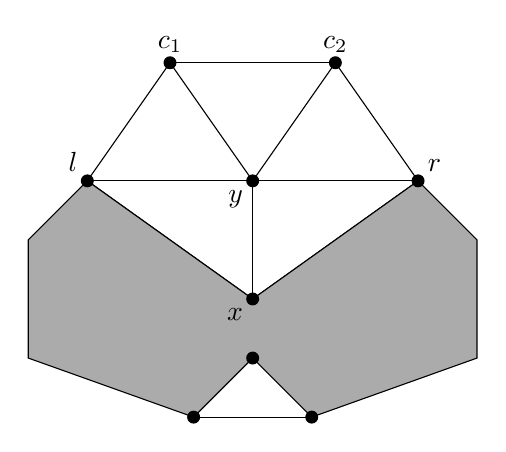
\begin{tikzpicture}[scale=1.5]
        \coordinate (c1) at (3,0);
        \coordinate (c2) at (3,1);
        \coordinate (l) at (1.6,1);
        \coordinate (r) at (4.4,1);
        \coordinate (v1) at (2.3,2);
        \coordinate (v2) at (3.7,2);
        \coordinate (b1) at (2.5,-1);
        \coordinate (b2) at (3,-0.5);
        \coordinate (b3) at (3.5,-1);

        \draw (c1) -- (l);
        \draw (c1) -- (r);
        \draw (c2) -- (l);
        \draw (c2) -- (r);
        \draw (c1) -- (c2);
        \draw (c2) -- (v1);
        \draw (c2) -- (v2);
        \draw (l) -- (v1);
        \draw (v1) -- (v2);
        \draw (v2) -- (r);
        \draw (b1) -- (b3);
        \draw[fill=black!33] (l) -- (1.1,0.5) -- (1.1,-0.5) -- (b1) -- (b2) --
        (b3) -- (4.9,-0.5) -- (4.9,0.5) -- (r) -- (c1) -- cycle;

        \node[below left] at (c1) {$x$};
        \node[below left] at (c2) {$y$};
        \node[above left] at (l) {$l$};
        \node[above right] at (r) {$r$};
        \node[above] at (v1) {$c_1$};
        \node[above] at (v2) {$c_2$};

        \foreach \v in {c1,c2,l,r,v1,v2,b1,b2,b3}
            \filldraw (\v) circle (0.05);
    \end{tikzpicture}
    \caption{2-leg center with fan above it}
    \label{fig:fan}
\end{figure}

In order to test whether $y$ is a basic 2-leg center, they compute
$\textsc{outer}(y)$, the number of neighbors of $x$ on the outer face, and
$\textsc{outerDeg3}(y)$, the number of neighbors of $x$ on the outer face with
degree equal to $3$.
If $\textsc{outer}(y) = \textsc{outerDeg3}(y) + 2$, that is if $y$ has exactly
two neighbors on the outer face with degree greater than $3$, then $y$ is a
basic 2-leg center.

Once again, consider Figure \ref{fig:fan}. Both $x$ and $y$ have exactly two
neighbors on the outer face with degree greater than 3, namely $l$ and $r$.
However, $x$ is not a basic 2-leg center.
If we additionally require $\textsc{outerDeg3}(x) > 0$ for $x$ to be a a basic
2-leg center, $x$ is no longer incorrectly identified as a basic 2-leg center,
and the implementation works.

\subsection{Drawing the Outer Face Correctly for Port Assignment}
When performing the port assignment, the fixed drawing of the outer face
determines which of the outer edges is subdivided and which rectangle occupies
the corners of the rectangular dual. For example, consider the 4-connected
component in Figure \ref{fig:outer:graph} with the drawing shown in Figure
\ref{fig:outer:outer}. As presented by \citet{ldrawing}, the edge $(b,c)$ is
subdivided and the rectangular dual is drawn as shown in Figure
\ref{fig:outer:paold}.

If there is now a virtual vertex (drawn in red) adjacent to $v$ in the face
bounded by $v,a,b$, this virtual vertex will be drawn as a rectangle with height
0 to the right of $v$.
Because of this, the edge $(v,b)$ will be assigned to the South port of $v$.
Now $b$ has to be drawn below $v$, $v$ below $a$ and $a$ below $b$.
This is impossible.
Instead, we draw the rectangular dual as shown in Figure \ref{fig:outer:panew}.
This way we avoid $b$ being drawn below $a$, which would conflict with the
assignment of the edge $(a,b)$ to the North port of $a$.

Analogously, if the outer face is drawn as in Figure \ref{fig:outer:outer2}, we
do not draw the rectangular dual like in Figure \ref{fig:outer:paold2} but
instead like in Figure \ref{fig:outer:panew2}.

\begin{figure}[ht]
    \center
    \begin{subfigure}{0.32\textwidth}
        \center
        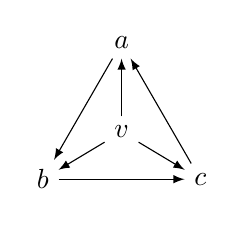
\begin{tikzpicture}[scale=2]
            \node (a) at (0.5,0.866) {$a$};
            \node (b) at (0,0) {$b$};
            \node (c) at (1,0) {$c$};
            \node (v) at (0.5,0.3) {$v$};
            \draw[->] (a) -- (b);
            \draw[->] (b) -- (c);
            \draw[->] (c) -- (a);
            \draw[->] (v) -- (a);
            \draw[->] (v) -- (b);
            \draw[->] (v) -- (c);
        \end{tikzpicture}
        \caption{4-connected component}
        \label{fig:outer:graph}
    \end{subfigure}
    \hfill
    \begin{subfigure}{0.15\textwidth}
        \center
        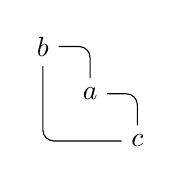
\begin{tikzpicture}[scale=0.6]
            \node (a) at (1,1) {$a$};
            \node (b) at (0,2) {$b$};
            \node (c) at (2,0) {$c$};
            \draw[rounded corners] (a) |- (b);
            \draw[rounded corners] (b) |- (c);
            \draw[rounded corners] (c) |- (a);
        \end{tikzpicture}
        \caption{Drawing of outer face}
        \label{fig:outer:outer}
    \end{subfigure}
    \hfill
    \begin{subfigure}{0.25\textwidth}
        \center
        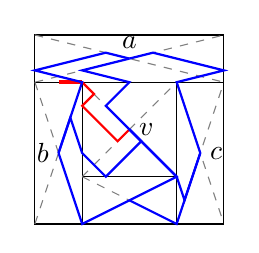
\begin{tikzpicture}[scale=0.6]
            \rectangle 0 3 4 4
            \rectangle 0 0 1 3
            \rectangle 3 0 4 3
            \rectangle 1 0 3 1
            \rectangle 1 1 3 3
            \coordinate[label={above:$a$}] (a) at (2,3.5);
            \coordinate[label={left:$b$}]  (b) at (0.5,1.5);
            \coordinate[label={right:$c$}] (c) at (3.5,1.5);
            \coordinate[label={right:$v$}] (v) at (2,2);
            \coordinate                    (d) at (2,0.5);
            \coordinate (virt) at (1,3);
            \draw[ultra thick,red] (virt) -- ++(-0.5,0);
            \draw[thick,red]  (v) -- ++(-0.25,-0.25) -- ++(-0.75,0.75) --
                ++(0.25,0.25) -- (virt);
            \draw[thick,blue] (a) -- (1.5,3.625) -- (0,3.25) -- (1,3) -- (b);
            \draw[thick,blue] (b) -- (1,0) -- (d);
            \draw[thick,blue] (d) -- (3,0) -- (c);
            \draw[thick,blue] (c) -- (3,3) -- (4,3.25) -- (2.5,3.625) -- (a);
            \draw[thick,blue] (v) -- ++(-0.5,0.5) -- ++(0.5,0.5) -- ++(-1,0.25)
                -- (a);
            \draw[thick,blue] (v) -- ++(+0.25,-0.25) -- ++(-0.75,-0.75) --
                ++(-0.5,0.5) -- ++(-0.25,0.75) -- (b);
            \draw[thick,blue] (v) -- (3,1) -- ++(1/6,-0.5) -- (c);
            \draw[thick,blue] (v) -- (3,1) -- (d);
        \end{tikzpicture}
        \caption{Port assignment}
        \label{fig:outer:paold}
    \end{subfigure}
    \hfill
    \begin{subfigure}{0.22\textwidth}
        \center
        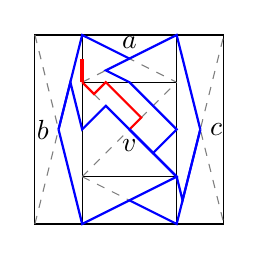
\begin{tikzpicture}[scale=0.6]
            \rectangle 1 3 3 4
            \rectangle 0 0 1 4
            \rectangle 3 0 4 4
            \rectangle 1 0 3 1
            \rectangle 1 1 3 3
            \coordinate[label={above:$a$}] (a) at (2,3.5);
            \coordinate[label={left:$b$}]  (b) at (0.5,2);
            \coordinate[label={right:$c$}] (c) at (3.5,2);
            \coordinate[label={below:$v$}] (v) at (2,2);
            \coordinate                    (d) at (2,0.5);
            \coordinate (virt) at (1,3);
            \draw[ultra thick,red] (virt) -- ++(0,0.5);
            \draw[thick,red]  (v) -- ++(0.25,0.25) -- ++(-0.75,0.75) --
                ++(-0.25,-0.25) -- (virt);
            \draw[thick,blue] (a) -- (1,4) -- (b);
            \draw[thick,blue] (b) -- (1,0) -- (d);
            \draw[thick,blue] (d) -- (3,0) -- (c);
            \draw[thick,blue] (c) -- (3,4) -- (a);
            \draw[thick,blue] (v) -- ++(0.5,-0.5) -- ++(0.5,0.5) -- ++(-1,1) --
                ++(-0.5,1/4) -- (a);
            \draw[thick,blue] (v) -- ++(-0.5,0.5) -- ++(-0.5,-0.5) --
                ++(-0.25,1) -- (b);
            \draw[thick,blue] (v) -- (3,1) -- ++(1/8,-0.5) -- (c);
            \draw[thick,blue] (v) -- (3,1) -- (d);
        \end{tikzpicture}
        \caption{Alternative}
        \label{fig:outer:panew}
    \end{subfigure}

    \medskip
    \begin{subfigure}{0.15\textwidth}
        \center
        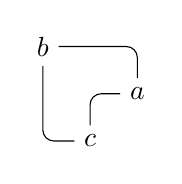
\begin{tikzpicture}[scale=0.6]
            \node (a) at (2,1) {$a$};
            \node (b) at (0,2) {$b$};
            \node (c) at (1,0) {$c$};
            \draw[rounded corners] (a) |- (b);
            \draw[rounded corners] (b) |- (c);
            \draw[rounded corners] (c) |- (a);
        \end{tikzpicture}
        \caption{Drawing of outer face}
        \label{fig:outer:outer2}
    \end{subfigure}
    \qquad
    \begin{subfigure}{0.25\textwidth}
        \center
        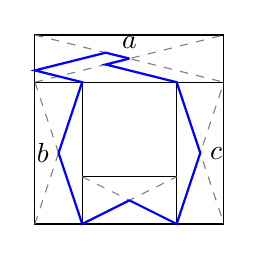
\begin{tikzpicture}[scale=0.6]
            \rectangle 0 3 4 4
            \rectangle 0 0 1 3
            \rectangle 3 0 4 3
            \rectangle 1 0 3 1
            \coordinate[label={above:$a$}] (a) at (2,3.5);
            \coordinate[label={left:$b$}]  (b) at (0.5,1.5);
            \coordinate[label={right:$c$}] (c) at (3.5,1.5);
            \coordinate                    (d) at (2,0.5);
            \draw[thick,blue] (a) -- (1.5,3.625) -- (0,3.25) -- (1,3) -- (b);
            \draw[thick,blue] (b) -- (1,0) -- (d);
            \draw[thick,blue] (d) -- (3,0) -- (c);
            \draw[thick,blue] (c) -- (3,3) -- ++(-3/2,3/8) -- (a);
        \end{tikzpicture}
        \caption{Port assignment}
        \label{fig:outer:paold2}
    \end{subfigure}
    \qquad
    \begin{subfigure}{0.22\textwidth}
        \center
        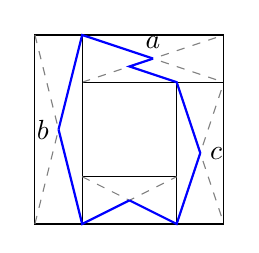
\begin{tikzpicture}[scale=0.6]
            \rectangle 1 3 4 4
            \rectangle 0 0 1 4
            \rectangle 3 0 4 3
            \rectangle 1 0 3 1
            \coordinate[label={above:$a$}] (a) at (2.5,3.5);
            \coordinate[label={left:$b$}]  (b) at (0.5,2);
            \coordinate[label={right:$c$}] (c) at (3.5,1.5);
            \coordinate                    (d) at (2,0.5);
            \draw[thick,blue] (a) -- (1,4) -- (b);
            \draw[thick,blue] (b) -- (1,0) -- (d);
            \draw[thick,blue] (d) -- (3,0) -- (c);
            \draw[thick,blue] (c) -- (3,3) -- ++(-1,1/3) -- (a);
        \end{tikzpicture}
        \caption{Alternative}
        \label{fig:outer:panew2}
    \end{subfigure}
    \caption{L-drawing of two particular 4-connected components}
    \label{fig:outer}
\end{figure}

\section{Discussion and Open Problems}\label{sec:end}
We sampled undirected plane triangulations uniformly at random.
However, the edge directions are not uniformly random.
For example, the graphs we sampled are always cycle-free with a single source
and a single sink on the outer face.
A solution to this shortcoming may be to reverse some randomly chosen edges of
the graph where bimodality permits it.
This approach would add sources and sinks on the inside of the graph as well as
cycles.
It is probably still not an adequate method of sampling bimodal triangulations
uniformly at random.

\citet{ldrawing} left as an open problem whether all bimodal graphs with 2-cycles
admit a planar embedding.
Our decomposition algorithm recognizes every triangle in the graph that has a
2-cycle as one of its sides as a separating triangle.
Therefore it was impossible to do any extensive testing on graphs with 2-cycles.
However, the port assignment algorithm without any modifications certainly does
not work correctly for
graphs with 2-cycles, as one can see in Figure \ref{fig:2cycle}.
There, the edge on the far left has three bends instead of the desired one bend.

\begin{figure}[ht]
    \center
    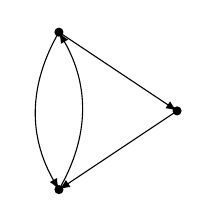
\begin{tikzpicture}
        \coordinate (a) at (0,2);
        \coordinate (b) at (0,0);
        \coordinate (c) at (1.5,1);
        \foreach \v in {a,b,c}
            \filldraw (\v) circle (0.05);

        \draw[->] (a) to[bend right] (b);
        \draw[->] (b) to[bend right] (a);
        \draw[->] (a) -- (c);
        \draw[->] (c) -- (b);
    \end{tikzpicture}
    \qquad
    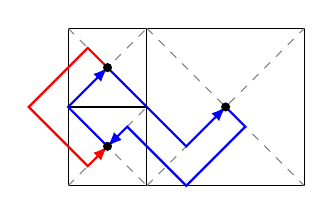
\begin{tikzpicture}
        \rectangle 0 0 1 1
        \rectangle 0 1 1 2
        \rectangle 1 0 3 2

        \draw[->,blue,thick] (0.5,0.5) -- (0,1) -- (0.5,1.5);
        \draw[->,red,thick] (0.5,1.5) -- (0.25,1.75) -- (-0.5,1)
            -- (0.25,0.25) -- (0.5,0.5);
        \draw[->,blue,thick] (0.5,1.5) -- (1.5,0.5) -- (2,1);
        \draw[->,blue,thick] (2,1) -- (2.25,0.75) -- (1.5,0)
            -- (0.75,0.75) -- (0.5,0.5);

        \filldraw (0.5,1.5) circle (0.05);
        \filldraw (0.5,0.5) circle (0.05);
        \filldraw (2,1) circle (0.05);
    \end{tikzpicture}
    \caption{Graph with 2-cycle and an incorrect port assignment}
    \label{fig:2cycle}
\end{figure}

In this particular case, the problem can be fixed by changing the embedding and
swapping the two edges of
the 2-cycle, but in more complex cases this may violate bimodality or even
4-modality.

\bibliographystyle{abbrvnat}
\bibliography{refs}

\end{document}
